\begin{refsection}
\chapter{The Incandescent Lamp and the Inverse Square Law}

\section*{Objectives}

\begin{enumerate}
\item To understand the current-voltage characteristics of an incandescent lamp's filament.
\item To understand the dependence of the lamp's power on the resistance of its filament.
\item To observe and understand the variation of intensity with distance for a point source.
\end{enumerate}




\section*{Introduction}

Thermal radiation is the conversion of thermal energy into electromagnetic energy. You should remember from earlier courses that the \textbf{temperature} of an object is a statistical property that -- at microscopic scales -- is a reflection of the average kinetic energy of the atoms or molecules present within that object. Thus, an increase in temperature would cause these atoms or molecules to start `jiggling' about more erratically (at least on an average). The higher the temperature, the more rapid this motion. This irregular thermal motion causes the charges that comprise the atoms and molecules to oscillate. 

A famous result in electrodynamics states that accelerating charges radiate electromagnetic radiation. Each oscillation at a particular frequency can be considered a tiny ``antenna'' that emits and receives electromagnetic radiation. Of course, since these oscillations are due to random collisions within the object, there is a \textit{continuous range} of possible frequencies of oscillations and thus of the emitted electromagnetic radiation. An object that emits radiation over a wide range of frequencies is known as a \textit{black body}, and the characteristic spectrum of radiation it produces is called black-body radiation. For example, as a piece of iron is heated to increasingly high temperatures, it first glows red, then yellow, and finally white. In short, all the colours of the visible spectrum are represented. In fact, the sensation of heat you get from the iron even before it begins to glow red is an indication of the emission of infrared radiation.

% \todo[inline]{Not happy with the definition of a blackbody...}


The spectrum of a blackbody was known quite well experimentally, however no theoretical approach could describe it accurately. There were two different laws, each of which fit the experimental data in different regimes, but neither of which explained the full spectrum. For low frequencies (or long wavelengths), the law was the ``Rayleigh-Jeans law'', while for high frequencies (or short wavelengths) it was known as ``Wein's displacement law''.

\begin{figure}[!htb]
\centering
\begin{subfigure}[b]{0.45\textwidth}
        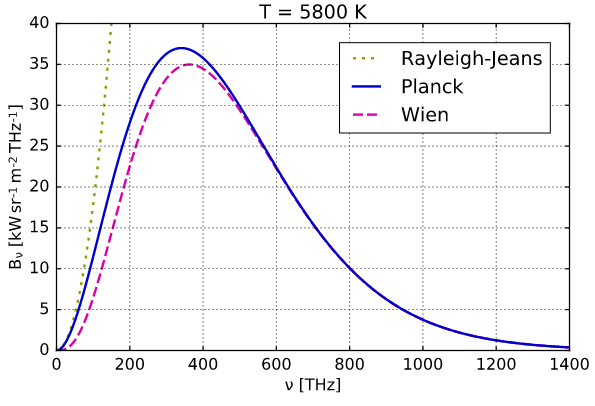
\includegraphics[width=\textwidth]{planck.png}
        \caption{Classical approximations}
        \label{planck_approx}
    \end{subfigure}%
    \begin{subfigure}[b]{0.45\textwidth}
        \hspace{0.5cm}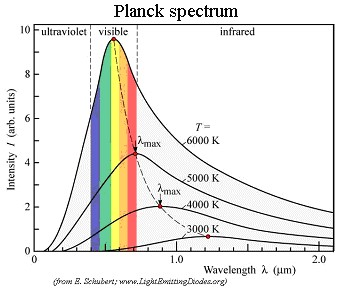
\includegraphics[width=0.8\textwidth]{planck_temp.jpg}
        \caption{Variation with temperature}
        \label{planck_temp}
    \end{subfigure}
\caption{The Planck Spectrum for Blackbodies}
\label{planck}
\end{figure}

The problem was solved by the German physicist Max Planck who realised that classical physics could not be used for such blackbody radiation, and thereby ushered in Quantum Mechanics by postulating that the energies were absorbed and emitted in specific quanta. The resulting spectrum was found to be characterised by one single parameter: the temperature of the object, and was found to fit a remarkable number of spectra from the sun to the Cosmic Microwave Background Radiation left as a remnant from the Big Bang.

\begin{question}
\paragraph{Question: } It is often said that the Cosmic Microwave Background Radiation has a ``temperature'' of 2.73 K. What do you think this means?
\end{question}


An incandescent lamp is composed of a wire filament protected from oxidation with a glass or fused quartz bulb that is filled with inert gas or a vacuum. If an electric current is passed through such a wire, it will begin to get heated. If the wire is heated to a sufficiently high temperature, it will give off light in the visible regime.  This is the basis of a resistive incandescent lamp. The high melting point of tungsten (3680 K) and its low vaporisation pressure makes it a suitable material to be used as the filament of almost all incandescent lamps. The brightness and the overall colour of emitted light depends on the temperature of the filament for a given lamp, which is a non-linear resistive element.

At the heart of the lamp is a resistive element, which should follow Ohm's Law. Thus, when a voltage is applied across the lamp, a current flows through it, and the two are related by 

\begin{equation}
    V = R I.
    \label{ohm}
\end{equation}

However, as more current flows through the the filament, it gets heated which in turn changes its resistance. Thus, a more appropriate way of writing the above equation for the filament is 

\begin{equation}
    V = R(I) I
\end{equation}

where $R$, despite being an ``instantaneous'' resistance, is not a constant value. Suppose we don't know the exact form of $R(I)$. One assumption might be to assume some sort of power law behaviour. Thus,

\begin{equation}
    V = K I^a
    \label{isl-Vpowerlaw}
\end{equation}

where $K$ and $a$ are constants, and $V$ is the voltage across the lamp and $I$ the current passing through it.

% Let us consider how the resistance varies as a function of temperature $T$. It is reasonable to assume that the temperature dependence of the resistance of the filament is given by

% \begin{equation}
%     R = R_0 \left( 1 + \alpha (T-T_0) \right)
% \end{equation}

% where $R_0$ is the resistance of the filament at the ambient temperature $T_0$, and $T$ is the temperature of the filament, and $\alpha$ is known as the temperature coefficient of resistance of the material.

% {\color{red}So this is my problem: I want to find the relation between temperature $T$ and current. I know the temperature $\Delta T \propto E_\text{rad} = m c \Delta T$, and the energy is $\int P \dd t$. 

% Now I need the power, and it's simply $VI$. I don't use $I^2R$ or $V^2/R$ since it doesn't give the true dependence on $I$, since $R(I)$. But since $R$ changes with time, and therefore so does $I$. Even if I assume the energy is simply $VIt$, this doesn't remove the problem, as now 

% \begin{equation}
%     \Delta T \propto VI
% \end{equation}

% Thus $R$ seems to depend on $V$ as well as $I$, and at this point I feel I'm doing something wrong.

% Alternatively, I could do the following: I say the energy (and hence $\Delta T$) is $\propto I$, and therefore $R(I) = R_0 (1 + \kappa I)$, which means that 

% \begin{equation}
%     V = R_0 (I + \kappa I^2)
% \end{equation}
% } 


% \todo[inline]{I'm increasingly coming to the conclusion that this entire experiment needs a rethink....}

Similarly, the power in the circuit can be calculated by the formula: 

\begin{equation}
    P = V I.
\end{equation}

For a normal resistor which follows Equation (\ref{ohm}) (known as Ohm's law), we could rewrite the equation as 

\begin{equation*}
    P = VI = I^2 R = \frac{V^2}{R},
\end{equation*}

however, in the case of an incandescent lamp where the ratio between the current and voltage is not a constant, this is no longer necessarily true. One finds for the resistive lamp, the empirical relation
\begin{equation*}
P = C R^n
\end{equation*}

where $P$ is the power supplied to the lamp, $R$ is the resistance of the filament of the lamp, and $n$ and $C$ are constants whose values depend on the material used for the filament of the lamp. The above relation yields better results when the temperature of the filament of the lamp is approximately above 1800 K for the given lamp. For such temperatures the resistance R of the lamp is found to be directly proportional to the absolute temperature T of the filament of the lamp.



\subsection*{Point sources}


A \textbf{point source} is a single identifiable localised source of, say, light. Such a source has negligible extent, distinguishing it from other source geometries, and are called point sources because in mathematical modelling, they can usually be approximated as a mathematical point to simplify analysis. The actual source need not be physically small, if its size is negligible relative to other length scales in the problem. For example, in astronomy, stars are routinely treated as point sources, even though they are in actuality much larger than the Earth.

For light or sound waves, a point source radiates the same intensity of radiation in all directions. That is, it has no preferred direction of radiation and radiates uniformly in all directions over a sphere centred on the source.

\begin{figure}
    \centering
    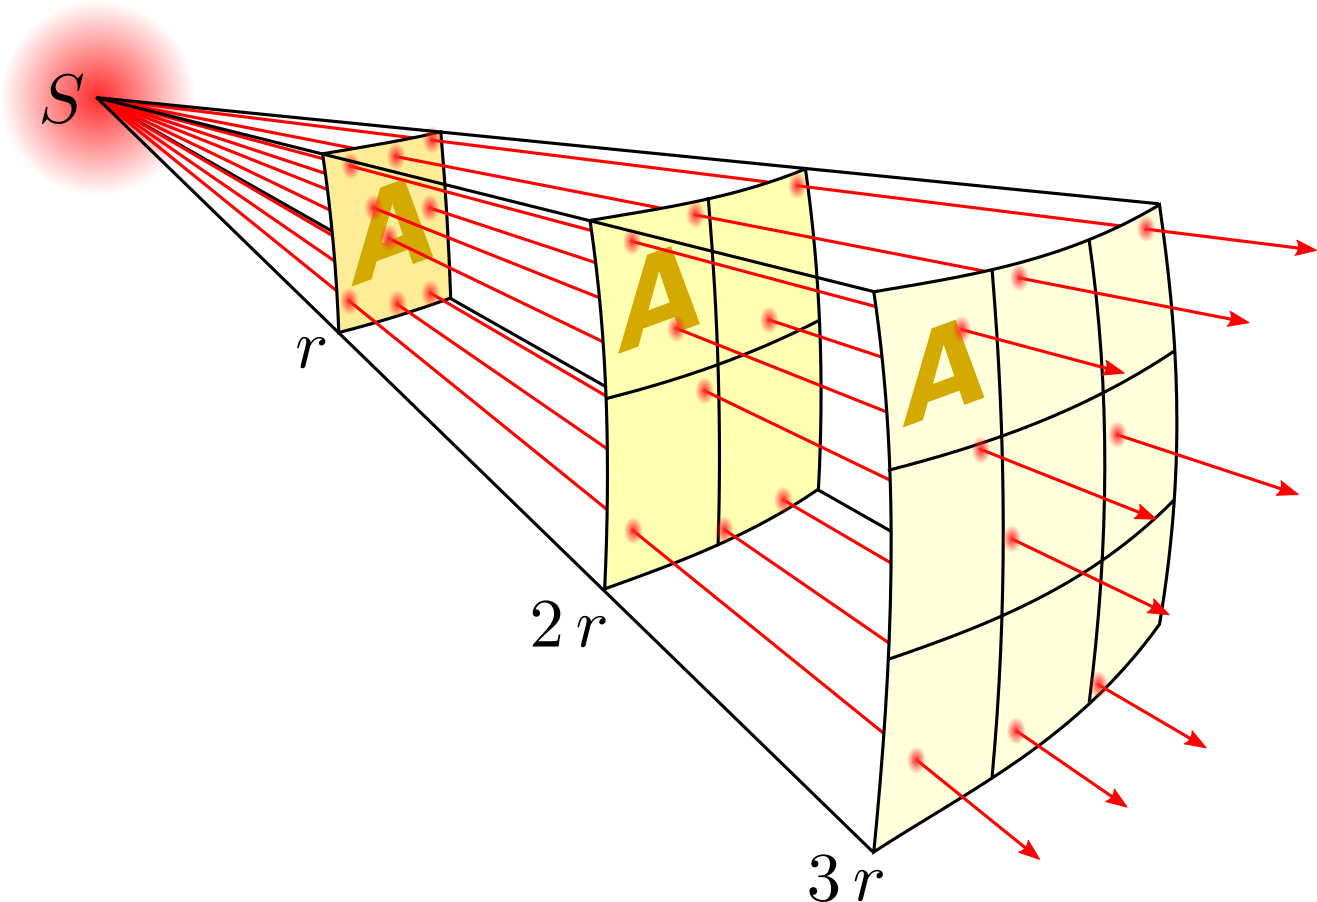
\includegraphics[width=0.5\textwidth]{figs/inversesquarelaw.png}
    \caption{Motivating the inverse square law: Suppose $S$ represents the light source, and the lines represent rays of light emanating from it. The total number of rays remains constant, as that represents the ``strength'' of the source. However, the density of these rays (that is, the rays per unit area) falls off with distance. If we imagine spheres of different radii ($r$, $2r$, and $3r$) centred around the position of $S$, then the density of rays on the surface of each of these spheres falls as the square of the radius, since the surface area of a sphere increases with the square of the radius. Thus, one would expect the intensity of the point-source to fall as an inverse-square law.}
    \label{fig:isl}
\end{figure}


\section*{Experimental Setup}

\subsection*{Apparatus}

\begin{enumerate}
\item A DC variable power supply (\textit{Optochem})
\item Two digital multimeters with probes (\textit{MECO 603} and \textit{Victor VC97})
\item A 12 V, 21W incandescent lamp
\item A stand to hold the lamp
\item A Resistor Ladder
\item Connecting cords
\item A convex lens
\item A photodiode

\end{enumerate}


\subsection*{Description}

\begin{description}
\item[Digital Multimeter (\textit{MECO 603}, \textit{Victor VC97})]

A multimeter is an instrument used to measure multiple parameters like voltage, current, and resistance. In this experiment you are given two digital multimeters (Models \textit{MECO - 603} and \textit{Victor VC97}).\footnote{The Victor multimeter has a greater current sensitivity.} You will have to use input sockets marked COM, V/$\Omega$ and mA (or A or 20A) for the required measurements. Note that there are two input sockets marked mA and 20A (10A for the Victor multimeter) for the current measurement. The socket marked mA may be used for measuring current below 250 mA and socket marked 20A (or 10A) may be used for measuring current up to 20 A (or 10A). You will have to select the appropriate function and the range using the rotary switch provided on the multimeter. The value of voltage or current is displayed on the LCD screen. The multimeter is turned off by turning the dial to the appropriate setting.

\item[Variable DC Power Supply (\textit{Optochem})]

The DC Variable Power Supply can either act as a source of constant voltage (CV), or constant current (CC). An ideal voltage source is one that produces a fixed voltage irrespective of the current the load (your circuit) demands of it. Of course, this is not realistic; the supply given to you can supply a maximum potential difference of 15V, and a maximum current of 2A.

The voltage and the current in the circuit can be changed using the three knobs: voltage coarse, voltage fine, and current. The given power supply also displays the values of the output voltage and current. Do not use these values since the multimeter will be more reliable. 

If the current knob is set to maximum, the supply acts as a constant voltage source. The constant voltage it supplies can be varied using the voltage knobs, and is independent of the load (your circuit) attached to it.\footnote{Similarly, if the voltage knob is set to maximum, the supply acts as a constant current source.}

\begin{imp}
If the current your circuit draws at any voltage is beyond 2A, the power supply will not be able to supply it. This could happen if you short the two terminals of the power supply (don't!) or connect it in any other way to a circuit that has effectively zero resistance. In this case, the power supply's output current will be 2A, indicating that it is providing the maximum current possible. Avoid this situation, as it could damage the power supply.
\end{imp}

\item[Photodiode]

A photodiode is a semiconductor device that converts light into an electrical current. The current is generated when photons of sufficient energy are absorbed in the photodiode, creating an electron-hole pair through the photoelectric effect.

\end{description}


\subsection*{Precautions}

\begin{itemize}
\item Do not apply a voltage more than 12 V to the lamp.
\item Clamp the lamp carefully on the retort stand so that the wires do not get shorted accidentally.
\item Use the digital multimeter for the measurement of DC voltage and current.  Choose the appropriate range for the measurement.
\item The incandescent lamp should not be kept connected to the power supply for long duration.
\item Passing more current through the multimeter's (250mA or 20A) sockets than they can handle will cause the fuses in the multimeter to burn out, leading to an open circuit. Use an appropriate resistance to limit the current in the circuit.
\item When drawing circuit diagrams use the standard symbols.
\item The digital multimeter and the DC power supply should be turned off if not in use.
\end{itemize}


\section*{Procedure}

\subsection*{Part A}

In this part, you will design an experiment to study the VI characteristics of an incandescent lamp. 

\begin{enumerate}
    \item  Begin by drawing the necessary circuit diagram, and connect the lamp to the power supply through a multimeter working as an ammeter. 
    
    \begin{imp} 
        Make sure you know how much current is flowing through the circuit so you know whether to use the 250mA or the 20A plugs on the multimeter. 
    \end{imp}
    
    \begin{question}
        \paragraph{Question:} How would you find the maximum resistance of a 12V, 21W lamp?
    \end{question}
    
    \item Connect a multimeter as a voltmeter across the lamp.
    
    \item Vary the voltage across the lamp and measure the current.
    
    \item Plot an appropriate graph to determine $K$ and $a$ in Equation (\ref{isl-Vpowerlaw}).
\end{enumerate}


\begin{question}
\paragraph{Question:} Describe qualitatively how you would expect the resistance of the lamp to vary with the current. Explain why you think this is the case.
\end{question}

\subsection*{Part B}

\begin{enumerate}
    \item Design an appropriate procedure to determine the value of $n$. You may use the  data collected in \textbf{Part A}, or you may perform new measurements.
    
    \item Plot an appropriate graph to determine $C$ and $n$.
\end{enumerate}


\subsection*{Part C}

In this part, you will design an experiment to create a point source and then study the variation of intensity of the light with distance.  For this you have to use the given photodiode with a digital multimeter to measure the intensity of light. We assume that the relation between the intensity of light incident on the sensing area of the photodiode and its output current is linear. 

\begin{enumerate}
    \item Use the converging lens to create a point source. You may use the screen with a hole in it to allow the passage of a small amount of light of this ``point source'' that may then be detected by the photodiode. The screen is now your point source. 
    
    \item Connect the output of the power supply to the given lamp and adjust the voltage applied to the lamp to be around 12 V. 
    
    \item Keep the photodiode initially as close as possible to the screen acting as your source. 
    
    \item Study the variation of current in the photodiode with the distance $d$ between the source and the photodiode. (You have to take readings for the value of $d$ varying from around 7.0 cm to around 50.0 cm.) You may have to correct your readings to account for the ambient light falling on the photodiode. 
    \item Plot an appropriate graph to show the variation of the intensity of light with distance $d$.
    
    \begin{question}
    \paragraph{Question:} What type of graph would be the most efficient to determine the variation of the intensity of light with distance? Why? 
    
    \paragraph{Question:} After plotting this graph, you may find that points below a certain value (say, 20.0 cm) do not behave as you would expect them to. Can you explain why this is the case?
    \end{question}
\end{enumerate}



\section*{References}

% \begin{enumerate}

% \item Justel, T. \href{https://www.fh-muenster.de/ciw/downloads/personal/juestel/juestel/4-InkohaerenteLichtquellen-Glueh-_und_Halogenlampen_english_-1.pdf}{Incandescent and Halogen Lamps}. Retrieved from \url{https://www.fh-muenster.de/ciw/downloads/personal/juestel/juestel/4-InkohaerenteLichtquellen-Glueh-_und_Halogenlampen_english_-1.pdf}.

% \item \href{https://www.elprocus.com/photodiode-working-principle-applications/}{Photodiode Working Principle, Characteristics and Applications}, ElProCus. Retrieved from \url{https://www.elprocus.com/photodiode-working-principle-applications/}.

% \end{enumerate}

% \nocite{justel_incoherent_nodate}
\nocite{schubert_light-emitting_2006}
\nocite{noauthor_photodiode_2016}

\printbibliography[heading=none]

\newpage
\end{refsection}